\documentclass[10pt,aspectratio=169]{beamer}

% ----- Encoding -----
% NOTE: babel[spanish] requiere texlive-lang-spanish (ausente en esta máquina);
% se omite para que compile en cualquier parte. El contenido es en español.
\usepackage[utf8]{inputenc}
\usepackage[T1]{fontenc}
\usepackage{lmodern}

% ----- Tema -----
\usetheme{Madrid}
\usecolortheme{whale}
\setbeamertemplate{navigation symbols}{}
\setbeamertemplate{caption}[numbered]
\setbeamerfont{frametitle}{size=\large}
\setbeamertemplate{itemize items}[circle]
\setbeamertemplate{section in toc}[sections numbered]

% ----- Paquetes -----
\usepackage{booktabs}
\usepackage{graphicx}
\usepackage{tikz}
\usetikzlibrary{arrows.meta, positioning, shapes.geometric}
\usepackage{xcolor}
\usepackage{listings}

\definecolor{awsorange}{RGB}{255,153,0}
\definecolor{darkblue}{RGB}{20,60,110}
\definecolor{softgray}{RGB}{245,245,245}
\definecolor{okgreen}{RGB}{0,120,60}
\definecolor{warnred}{RGB}{170,30,30}

\lstset{
  basicstyle=\ttfamily\scriptsize,
  backgroundcolor=\color{softgray},
  frame=single,
  framerule=0pt,
  breaklines=true,
  columns=fullflexible,
  keepspaces=true,
  aboveskip=4pt,
  belowskip=4pt,
}

% ----- Título -----
\title[GOES en AWS]{Datos satelitales GOES desde AWS}
\subtitle{Metodología, arquitectura para un visor en tiempo real y costos}
\author{Esteban Ladino Nieto}
\institute[Uniandes]{Universidad de los Andes \\ \small Ing.\ Industrial \& Ing.\ Mecánica}
\date{\today}

\begin{document}

% ================================================================
\begin{frame}
  \titlepage
\end{frame}

% ================================================================
\begin{frame}{Contenido}
  \tableofcontents
\end{frame}

% ================================================================
\section{Contexto y punto de partida}
% ================================================================

\begin{frame}{Contexto: de dónde sale este flujo}
  \begin{columns}[T]
    \begin{column}{0.52\textwidth}
      \textbf{Dos proyectos de grado (2025--2026)}
      \begin{itemize}
        \item \textbf{Ing.\ Mecánica} --- Dir.\ Andrés González Mancera\\
              \small Pronóstico multifuente de irradiancia (GHI) a 60~min,
              estación en Bogotá.
        \item \textbf{Ing.\ Industrial} --- Dir.\ Alejandra Tabares\\
              \small Comparación de arquitecturas para pronóstico solar,
              planta FV en El~Paso (César).
      \end{itemize}
      \vspace{0.4em}
      Ambos necesitaban miles de horas de imágenes GOES de forma reproducible.
    \end{column}
    \begin{column}{0.44\textwidth}
      \begin{block}{Productos GOES usados}
        \begin{itemize}
          \item \texttt{ABI-L2-MCMIPF}\\
                \small 16 canales espectrales, hasta 6 fotogramas/hora
          \item \texttt{ABI-L2-DSRF}\\
                \small Irradiancia de onda corta en superficie
        \end{itemize}
      \end{block}
      \begin{alertblock}{Escala ingerida}
        \small feb 2022 -- abr 2025 $\approx$ \textbf{27.000 horas}
        $\times$ 2 productos.
      \end{alertblock}
    \end{column}
  \end{columns}
\end{frame}

% ================================================================
\begin{frame}{Importante: dos problemas distintos}
  \begin{columns}[T]
    \begin{column}{0.47\textwidth}
      \begin{block}{Lo que yo construí}
        \textbf{Ingesta histórica masiva}
        \begin{itemize}\small
          \item Miles de horas \emph{del pasado}
          \item Salida: arreglos \texttt{.npz} para \textbf{entrenar modelos}
          \item Optimizado para: reintentos, cobertura completa, costo por lote
          \item La latencia \textbf{no importa}
        \end{itemize}
      \end{block}
    \end{column}
    \begin{column}{0.47\textwidth}
      \begin{block}{Lo que ustedes necesitan}
        \textbf{Visor en tiempo casi real}
        \begin{itemize}\small
          \item \emph{La imagen más reciente}, siempre
          \item Salida: \textbf{PNG/JPEG para mostrar} en el dashboard
          \item Optimizado para: latencia, caché, costo por visita
          \item El histórico \textbf{no importa} (o solo unas horas)
        \end{itemize}
      \end{block}
    \end{column}
  \end{columns}
  \vspace{0.5em}
  \begin{alertblock}{Qué se transfiere y qué no}
    \small
    \textcolor{okgreen}{\textbf{Sirve igual:}} cómo se localizan los archivos en S3,
    el recorte geográfico, la Lambda con Docker, los permisos, la lógica de verificación.\\
    \textcolor{warnred}{\textbf{Cambia:}} el disparador (cron/evento en vez de barrido),
    el formato de salida (imagen en vez de tensor), el almacenamiento (ventana móvil) y
    la entrega (CDN).
  \end{alertblock}
\end{frame}

% ================================================================
\section{Fundamentos: los datos GOES en AWS}
% ================================================================

\begin{frame}[fragile]{Cómo están organizados los datos en AWS Open Data}
  El bucket público sigue una convención estricta que hay que reproducir
  para construir el \emph{prefix}:

\begin{lstlisting}
s3://noaa-goes19/ABI-L2-<PRODUCTO>/<YYYY>/<DOY>/<HH>/
    OR_ABI-L2-<PRODUCTO>-M6_G19_s<YYYYDOYHHMMSSS>_e<...>_c<...>.nc
\end{lstlisting}

  \begin{columns}[T]
    \begin{column}{0.48\textwidth}
      \begin{block}{Detalles que cuestan tiempo}
        \small
        \begin{itemize}\small
          \item \texttt{DOY} = \textbf{día juliano} (001--366), no el mes
          \item \texttt{s} = inicio de escaneo, \texttt{e} = fin,
                \texttt{c} = creación. \textbf{Ordenar por \texttt{s}}
          \item Todo en \textbf{UTC}
        \end{itemize}
      \end{block}
    \end{column}
    \begin{column}{0.48\textwidth}
      \begin{block}{Satélite operativo}
        \small
        \textbf{GOES-16} $\to$ histórico (hasta abr.\ 2025)\\
        \textbf{GOES-19} $\to$ GOES-East \textbf{actual}\\[0.2em]
        Para un visor en vivo: \texttt{noaa-goes19}.
      \end{block}
    \end{column}
  \end{columns}

  \vspace{0.3em}
  \footnotesize
  \textbf{Nota de acceso:} en mi flujo el acceso se configuró con
  \emph{Requester Pays} (\texttt{--request-payer requester} en CLI,
  \texttt{RequestPayer='requester'} en \texttt{boto3}). Conviene verificarlo al
  inicio: si aplica y no se pasa el flag, la petición falla con
  \texttt{AccessDenied}.
\end{frame}

% ================================================================
\begin{frame}{Qué producto pedir según lo que se quiere mostrar}
  \begin{table}
    \centering\footnotesize
    \begin{tabular}{@{}lll@{}}
      \toprule
      \textbf{Producto} & \textbf{Qué trae} & \textbf{Para qué sirve} \\
      \midrule
      \texttt{ABI-L2-CMIPF} & Un canal, full disk & Imagen simple de un canal \\
      \texttt{ABI-L2-MCMIPF} & \textbf{16 canales}, full disk & Compuestos RGB, ML \\
      \texttt{ABI-L2-DSRF} & Irradiancia en superficie & Energía solar (W/m$^2$) \\
      \texttt{ABI-L1b-RadF} & Radiancias crudas & Si necesitan calibración propia \\
      \bottomrule
    \end{tabular}
  \end{table}

  \vspace{0.3em}
  \begin{columns}[T]
    \begin{column}{0.48\textwidth}
      \begin{block}{Cadencia (Modo 6)}
        \small
        \textbf{Full disk (F)}: cada \textbf{10 min}\\
        \textbf{CONUS (C)}: cada 5 min --- \emph{no cubre Colombia}\\
        \textbf{Mesoescala (M)}: cada 1 min, ventana móvil\\[0.3em]
        Para Colombia: \textbf{full disk}, 10 min.
      \end{block}
    \end{column}
    \begin{column}{0.48\textwidth}
      \begin{block}{Sugerencia para el dashboard}
        \small
        \textbf{MCMIPF} es el más versátil: con un solo archivo por instante
        tienen todos los canales para armar la vista visible (día), la
        infrarroja (noche) y, si quieren, superponer la irradiancia
        de \texttt{DSRF}.
      \end{block}
    \end{column}
  \end{columns}
\end{frame}

% ================================================================
\section{Arquitectura para el visor en tiempo real}
% ================================================================

\begin{frame}{Tres caminos posibles (de menor a mayor esfuerzo)}
  \begin{columns}[T]
    \begin{column}{0.31\textwidth}
      \begin{block}{A. Embeber lo existente}
        \small
        Usar visores públicos ya renderizados (NOAA STAR, RAMMB/CIRA SLIDER)
        dentro de una pestaña.\\[0.3em]
        \textcolor{okgreen}{\textbf{+}} Costo casi nulo, inmediato\\
        \textcolor{warnred}{\textbf{--}} Sin control de encuadre ni de marca;
        sujeto a términos de uso de terceros
      \end{block}
    \end{column}
    \begin{column}{0.31\textwidth}
      \begin{block}{B. Cron $\to$ Lambda \textcolor{okgreen}{(recomendado)}}
        \small
        Cada 10 min, una Lambda busca el archivo más reciente, renderiza y
        publica un PNG en S3.\\[0.3em]
        \textcolor{okgreen}{\textbf{+}} Control total, simple, barato\\
        \textcolor{warnred}{\textbf{--}} Latencia de hasta un ciclo
      \end{block}
    \end{column}
    \begin{column}{0.31\textwidth}
      \begin{block}{C. Dirigido por eventos}
        \small
        Suscribirse a las notificaciones de objeto nuevo que publica NOAA
        (SNS) y renderizar al instante.\\[0.3em]
        \textcolor{okgreen}{\textbf{+}} Latencia mínima\\
        \textcolor{warnred}{\textbf{--}} Más piezas que configurar
      \end{block}
    \end{column}
  \end{columns}
  \vspace{0.5em}
  \begin{alertblock}{Mi recomendación}
    \small
    Empezar por \textbf{B}. Es la que mejor relación esfuerzo/control tiene, y
    migrar a \textbf{C} después es un cambio pequeño (se reemplaza el
    disparador, el resto del código queda igual). Si el objetivo fuera solo
    ``ver la nube'', \textbf{A} puede ser suficiente y honesto reconocerlo.
  \end{alertblock}
\end{frame}

% ================================================================
\begin{frame}{Arquitectura recomendada (opción B)}
  \begin{center}
  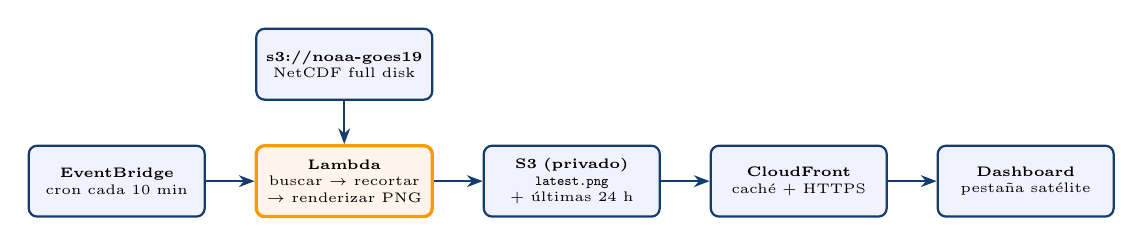
\begin{tikzpicture}[
      node distance=0.7cm and 0.62cm,
      box/.style={rectangle, rounded corners=3pt, draw=darkblue, thick,
                  fill=blue!5, align=center, minimum height=0.9cm,
                  text width=2.0cm, font=\tiny},
      awsbox/.style={rectangle, rounded corners=3pt, draw=awsorange, very thick,
                  fill=orange!8, align=center, minimum height=0.9cm,
                  text width=2.0cm, font=\tiny},
      arr/.style={-{Stealth[length=2mm]}, thick, draw=darkblue}
    ]
    \node[box] (sched) {\textbf{EventBridge}\\ cron cada 10 min};
    \node[awsbox, right=of sched] (lambda) {\textbf{Lambda}\\ buscar $\to$ recortar\\ $\to$ renderizar PNG};
    \node[box, above=0.55cm of lambda] (noaa) {\textbf{s3://noaa-goes19}\\ NetCDF full disk};
    \node[box, right=of lambda] (s3) {\textbf{S3 (privado)}\\ \texttt{latest.png}\\ + últimas 24 h};
    \node[box, right=of s3] (cf) {\textbf{CloudFront}\\ caché + HTTPS};
    \node[box, right=of cf] (dash) {\textbf{Dashboard}\\ pestaña satélite};

    \draw[arr] (sched) -- (lambda);
    \draw[arr] (noaa) -- (lambda);
    \draw[arr] (lambda) -- (s3);
    \draw[arr] (s3) -- (cf);
    \draw[arr] (cf) -- (dash);
  \end{tikzpicture}
  \end{center}

  \vspace{-0.3em}
  \begin{columns}[T]
    \begin{column}{0.33\textwidth}
      \footnotesize
      \textbf{Por qué CloudFront}\\
      Si 200 personas abren la pestaña, S3 sirve el PNG \textbf{una vez} y el
      CDN atiende el resto. Es lo que mantiene el costo plano.
    \end{column}
    \begin{column}{0.33\textwidth}
      \footnotesize
      \textbf{Ventana móvil}\\
      Regla de ciclo de vida en S3: borrar frames con más de 24--48~h.
      Almacenamiento acotado y permite animar el bucle.
    \end{column}
    \begin{column}{0.31\textwidth}
      \footnotesize
      \textbf{Región}\\
      \texttt{us-east-1}: misma región del bucket público $\Rightarrow$ sin
      costo de transferencia entre regiones.
    \end{column}
  \end{columns}
\end{frame}

% ================================================================
\begin{frame}[fragile]{Paso a paso (opción B)}
  \begin{enumerate}\small
    \item \textbf{Crear el bucket} de salida (privado) en \texttt{us-east-1}.
    \item \textbf{Construir la imagen Docker} de la Lambda con
          \texttt{boto3}, \texttt{xarray}, \texttt{netCDF4}, \texttt{numpy},
          \texttt{matplotlib}/\texttt{Pillow}; publicarla en \textbf{ECR}.
    \item \textbf{Crear la Lambda} (\texttt{--package-type Image},
          $\sim$2048~MB RAM, \texttt{/tmp} amplio, \emph{timeout} $\ge$ 2~min).
    \item \textbf{Rol IAM}: leer el bucket de NOAA, escribir en el bucket propio,
          escribir logs en CloudWatch.
    \item \textbf{Programar} con EventBridge Scheduler: \texttt{rate(10 minutes)}.
    \item \textbf{Publicar} con CloudFront apuntando al bucket
          (OAC, sin exponer el bucket directamente).
    \item \textbf{Regla de ciclo de vida} para expirar frames antiguos.
  \end{enumerate}

  \vspace{0.2em}
\begin{lstlisting}
# Buscar el granulo mas reciente de la hora actual (UTC)
prefix = f"ABI-L2-MCMIPF/{yyyy}/{doy}/{hh}/"
objs = s3.list_objects_v2(Bucket="noaa-goes19", Prefix=prefix)
latest = max(objs["Contents"], key=lambda o: o["Key"])  # ordena por _s...
\end{lstlisting}
  \footnotesize
  \textcolor{warnred}{Ojo:} al inicio de cada hora UTC el prefijo nuevo está
  vacío por unos minutos $\Rightarrow$ si no hay objetos, retroceder a la hora
  anterior.
\end{frame}

% ================================================================
\begin{frame}{Del NetCDF a una imagen que se vea bien}
  \begin{columns}[T]
    \begin{column}{0.5\textwidth}
      \begin{block}{Lo mínimo que funciona}
        \small
        \begin{enumerate}\small
          \item Leer el canal deseado con \texttt{xarray}
          \item Recortar la región (Colombia)
          \item Escalar valores a 0--255
          \item Guardar PNG con \texttt{Pillow}
        \end{enumerate}
      \end{block}
      \begin{alertblock}{Día y noche}
        \small
        Los canales \textbf{visibles se apagan de noche}. Un visor 24/7 debe
        conmutar: visible de día (\texttt{C02}), \textbf{infrarrojo}
        (\texttt{C13}) de noche --- o mezclar según el ángulo solar.
      \end{alertblock}
    \end{column}
    \begin{column}{0.48\textwidth}
      \begin{block}{Si quieren color ``realista''}
        \small
        El ABI \textbf{no tiene banda verde}. El color verdadero se
        \emph{sintetiza} combinando \texttt{C01} (azul), \texttt{C02} (rojo) y
        \texttt{C03} (veggie).\\[0.3em]
        Productos como \emph{GeoColor} (lo que se ve en la página de NOAA) son
        recetas elaboradas con corrección atmosférica y capas nocturnas.
      \end{block}
      \footnotesize
      \textbf{Consejo:} empezar con un canal en escala de grises. Se ve
      profesional, es robusto y evita semanas de ajuste de color. El RGB puede
      venir después.
    \end{column}
  \end{columns}
\end{frame}

% ================================================================
\begin{frame}{Valor agregado: lo que la página de NOAA no puede darles}
  \begin{columns}[T]
    \begin{column}{0.5\textwidth}
      Si van a montar infraestructura propia, que sea por algo que un visor
      público no ofrece:
      \begin{itemize}\small
        \item \textbf{Superponer sus propios datos}: ubicación del edificio,
              y la lectura en vivo de la planta FV y la estación meteorológica.
        \item \textbf{Encuadre propio}: la vecindad de Bogotá, no todo el
              hemisferio.
        \item \textbf{Correlación visual}: ver la nube entrando \emph{y} la
              caída de potencia en la misma pantalla.
        \item \textbf{Serie corta propia}: bucle de las últimas horas.
      \end{itemize}
    \end{column}
    \begin{column}{0.48\textwidth}
      \begin{block}{Un paso más (opcional)}
        \small
        Con \texttt{DSRF} pueden mostrar un \textbf{mapa de irradiancia en
        superficie} (W/m$^2$) y compararlo directamente con lo que mide la
        estación del edificio. Es una vista mucho más informativa para una
        comunidad de ingeniería que una imagen de nubes.
      \end{block}
      \begin{block}{Y más adelante}
        \small
        Sobre esa misma base se puede añadir el \textbf{pronóstico} a 1--6~h
        (lo que trabajo en mi tesis) como una capa adicional del dashboard.
      \end{block}
    \end{column}
  \end{columns}
\end{frame}

% ================================================================
\section{Costos y presupuesto}
% ================================================================

\begin{frame}{Costos estimados}
  \begin{columns}[T]
    \begin{column}{0.52\textwidth}
      \begin{block}{Visor en tiempo real (opción B)}
        \small
        Cada 10 min $\Rightarrow$ $\approx$ \textbf{4.400 invocaciones/mes}.
        \begin{itemize}\footnotesize
          \item Lambda: pocos USD/mes (a menudo dentro de capa gratuita)
          \item S3: ventana de 24--48~h $\Rightarrow$ almacenamiento mínimo
          \item CloudFront: depende de visitas; con caché es bajo
        \end{itemize}
        \vspace{0.2em}
        \textcolor{darkblue}{\textbf{Orden de magnitud: decenas de USD/mes}},
        no cientos --- \emph{si} se usa caché.
      \end{block}
    \end{column}
    \begin{column}{0.44\textwidth}
      \begin{block}{Ingesta histórica (mi caso)}
        \small
        \textbf{USD 15--50} por el proceso completo, según rango de fechas y
        paralelismo.\\[0.2em]
        \footnotesize
        Referencia: una semana de prueba (7~días $\times$ 24~h)
        $\approx$ 168 invocaciones.
      \end{block}
      \begin{alertblock}{El costo que sorprende}
        \small
        Servir la imagen \textbf{sin caché}: si cada visita golpea S3
        directamente, el costo crece con los usuarios. Con CloudFront se
        aplana.
      \end{alertblock}
    \end{column}
  \end{columns}
\end{frame}

% ================================================================
\begin{frame}{Cómo armar el presupuesto formal}
  \begin{columns}[T]
    \begin{column}{0.55\textwidth}
      \textbf{AWS Pricing Calculator} --- \texttt{calculator.aws}
      \begin{block}{Servicios a incluir}
        \small
        \begin{enumerate}\small
          \item \textbf{Lambda}: n.º de solicitudes/mes y duración media
                ($\sim$4.400 invocaciones, estimar segundos por ejecución)
          \item \textbf{S3}: GB almacenados + solicitudes PUT/GET
          \item \textbf{CloudFront}: GB transferidos + solicitudes
          \item \textbf{ECR}: almacenamiento de la imagen (centavos)
          \item \textbf{CloudWatch}: logs
        \end{enumerate}
      \end{block}
      \small
      Genera un enlace compartible y un PDF --- útil para justificar el rubro
      ante el Departamento.
    \end{column}
    \begin{column}{0.42\textwidth}
      \begin{block}{Buenas prácticas de control}
        \small
        \begin{itemize}\small
          \item \textbf{AWS Budgets} con alerta por correo (p.\,ej.\ al 80\%
                del tope) --- \emph{esto es lo que evita sustos}
          \item Etiquetar recursos por proyecto para rastrear el gasto
          \item Revisar \textbf{Cost Explorer} la primera semana
          \item Considerar créditos de \textbf{AWS Educate / Research}
        \end{itemize}
      \end{block}
      \footnotesize
      \textcolor{warnred}{Sugerencia:} pongan el tope de presupuesto
      \emph{antes} de encender el cron, no después.
    \end{column}
  \end{columns}
\end{frame}

% ================================================================
\section{Recomendaciones y lecciones}
% ================================================================

\begin{frame}{Recomendaciones para empezar}
  \begin{enumerate}
    \item \textbf{Prueben con una sola imagen, a mano, antes de automatizar.}\\
          \small Descarguen un NetCDF con la CLI y ábranlo en un notebook.
          Si logran renderizar \emph{una} imagen, lo demás es plomería.
    \item \textbf{Trabajen en \texttt{us-east-1}.}\\
          \small Es donde vive el bucket público; fuera de ahí se paga transferencia.
    \item \textbf{Definan primero el encuadre y la resolución de salida.}\\
          \small Determina el peso del PNG y la fluidez del dashboard.
    \item \textbf{Caché desde el principio.}\\
          \small Es la diferencia entre un costo plano y uno que crece con las visitas.
    \item \textbf{Ventana móvil, no archivo histórico.}\\
          \small Para un visor no necesitan guardar años. Regla de ciclo de vida y listo.
    \item \textbf{Presupuesto y alerta antes de encender el cron.}\\
          \small AWS Budgets con notificación por correo.
    \item \textbf{Manejen el caso ``todavía no hay imagen''.}\\
          \small Publiquen siempre un \texttt{latest.png} válido: el dashboard nunca
          debe quedar en blanco por un granulo que se retrasó.
  \end{enumerate}
\end{frame}

% ================================================================
\begin{frame}{Lecciones aprendidas (lo que me costó tiempo)}
  \begin{columns}[T]
    \begin{column}{0.5\textwidth}
      \begin{alertblock}{1. Zonas horarias: el error más caro}
        \small
        Las imágenes GOES están en \textbf{UTC real}. Los datos de estación
        suelen venir en hora local --- a veces \textbf{mal etiquetados como UTC}.\\[0.3em]
        En mi caso un archivo traía sufijo \texttt{+00:00} siendo hora local:
        \textbf{5 horas de desfase}, sin generar ningún error.
      \end{alertblock}
      \footnotesize
      \textbf{Cómo detectarlo:} el pico diario de irradiancia debe caer cerca
      del mediodía solar ($\approx$ 16--17~UTC en Colombia). Si aparece a otra
      hora, hay desfase. \textcolor{warnred}{Crítico si van a cruzar la imagen
      con los datos de la planta.}
    \end{column}
    \begin{column}{0.48\textwidth}
      \begin{block}{2. Los binarios nativos mandan}
        \small
        \texttt{netCDF4}/\texttt{xarray} traen librerías compiladas
        $\Rightarrow$ \textbf{imagen Docker}, no \emph{layers}. Ahorra días.
      \end{block}
      \begin{block}{3. Memoria y \texttt{/tmp} de Lambda}
        \small
        Un full disk pesa cientos de MB: 2~GB de RAM y 4~GB de \texttt{/tmp}
        fue la configuración estable.
      \end{block}
      \begin{block}{4. Huecos que no son bugs}
        \small
        Algunas horas simplemente \textbf{no existen} en el dataset público.
        Verifíquenlo antes de perseguir un error inexistente.
      \end{block}
    \end{column}
  \end{columns}
\end{frame}

% ================================================================
\section{Contexto: mi trabajo actual}
% ================================================================

\begin{frame}{En qué estoy trabajando ahora}
  \textbf{Tesis actual} (Dir.\ Alejandra Tabares): pronóstico de GHI a 1, 3 y 6~horas
  con \textbf{cuantificación de incertidumbre}, en dos sitios de clima contrastante.

  \vspace{0.4em}
  \begin{columns}[T]
    \begin{column}{0.48\textwidth}
      \begin{block}{Del ConvLSTM a los grafos}
        \small
        \textbf{ResNet-LSTM}: trata cada parche como imagen (convolución +
        submuestreo) y una LSTM sobre la secuencia.\\[0.35em]
        \textbf{GraphSAGE-LSTM} (lo nuevo): trata el parche como un
        \textbf{grafo de píxeles}; cada píxel agrega información de sus vecinos
        con pesos por distancia, \emph{sin} reducir resolución.
      \end{block}
    \end{column}
    \begin{column}{0.48\textwidth}
      \begin{block}{Por qué un grafo}
        \small
        Una convolución desliza el \emph{mismo} filtro por toda la imagen. El
        grafo permite tratar distinto el centro del parche (la estación) y la
        periferia (por donde entran las nubes).
      \end{block}
      \begin{alertblock}{Ablación honesta}
        \small
        Comparo contra un \textbf{FlatMLP} que promedia el parche y descarta la
        estructura espacial: mide cuánto aporta realmente lo espacial.
      \end{alertblock}
    \end{column}
  \end{columns}
\end{frame}

% ================================================================
\begin{frame}{Cuantificación de incertidumbre}
  \textbf{La idea:} un pronóstico puntual no dice \emph{si se puede confiar en él}.
  No basta un intervalo: hay que saber \textbf{por qué} es incierto.

  \vspace{0.4em}
  \begin{columns}[T]
    \begin{column}{0.48\textwidth}
      \begin{block}{Aleatoria $\sigma_a^2$}
        \small
        Ruido \textbf{irreducible} del proceso físico (la nube es
        intrínsecamente impredecible).\\[0.2em]
        \textcolor{darkblue}{$\Rightarrow$ margen de reserva.}
      \end{block}
    \end{column}
    \begin{column}{0.48\textwidth}
      \begin{block}{Epistémica $\sigma_\text{epi}^2$}
        \small
        Ignorancia \textbf{reducible}: condiciones que el modelo ha visto poco.\\[0.2em]
        \textcolor{darkblue}{$\Rightarrow$ recolectar datos, reentrenar.}
      \end{block}
    \end{column}
  \end{columns}

  \vspace{0.4em}
  \begin{block}{Enfoque: entrenamiento cooperativo secuencial (Yi \& Bessa, 2025)}
    \small
    En vez de entrenar media y varianza juntas (lo que produce varianzas
    sobreconfiadas), se entrenan \textbf{en secuencia}:
    \textbf{(1)} red de media (congelada) $\to$
    \textbf{(2)} red de varianza sobre los residuos $\to$
    \textbf{(3)} muestreo de la posterior de pesos para lo epistémico.\\[0.3em]
    \footnotesize
    \textcolor{warnred}{Estado real:} pasos 1--2 funcionando y validados; el paso 3
    es un problema abierto --- la cadena no converge a una posterior estable en
    redes sobreparametrizadas.
  \end{block}
\end{frame}

% ================================================================
\begin{frame}{Un resultado que puede interesarles}
  \begin{columns}[T]
    \begin{column}{0.55\textwidth}
      \begin{block}{El clima cambia la respuesta}
        \small
        En el sitio de \textbf{montaña} (Bogotá), un modelo \emph{sin ninguna}
        estructura espacial alcanza casi el mismo desempeño que los modelos
        espaciales a 6~horas.\\[0.3em]
        $\Rightarrow$ El ciclo diurno regular y la convección local dejan poco
        margen a la información espacial del satélite.\\[0.3em]
        En \textbf{tierra caliente} (El~Paso) el aporte satelital es
        sustancialmente mayor.
      \end{block}
    \end{column}
    \begin{column}{0.42\textwidth}
      \begin{alertblock}{Lección transferible}
        \small
        \textbf{Más datos satelitales no siempre $=$ mejor pronóstico.}
        Conviene medir contra una línea base simple \emph{antes} de invertir en
        arquitecturas complejas.
      \end{alertblock}
      \footnotesize
      Y siempre comparar contra \textbf{persistencia}
      ($\hat{y}_{t+H} = y_t$): es sorprendentemente difícil de superar a
      horizontes cortos.
    \end{column}
  \end{columns}
\end{frame}

% ================================================================
\section{Cierre}
% ================================================================

\begin{frame}{Resumen y próximos pasos}
  \begin{columns}[T]
    \begin{column}{0.48\textwidth}
      \textbf{Para el visor, en una frase}
      \begin{block}{}
        \small
        Una \textbf{Lambda programada cada 10 min} que toma el granulo más
        reciente de \texttt{noaa-goes19}, lo recorta sobre Colombia, lo
        renderiza a PNG y lo publica en \textbf{S3 detrás de CloudFront}.
      \end{block}
      \vspace{0.2em}
      \textbf{Lo que más ahorra tiempo}
      \begin{itemize}\small
        \item Renderizar \emph{una} imagen a mano primero
        \item Escala de grises antes que RGB
        \item Presupuesto y alerta antes del cron
      \end{itemize}
    \end{column}
    \begin{column}{0.48\textwidth}
      \textbf{Con gusto puedo compartir}
      \begin{itemize}\small
        \item Los instructivos completos (anexos de ambas tesis) con el código
              de la Lambda y la configuración paso a paso
        \item Los repositorios de los dos proyectos
        \item Acompañarlos en el montaje inicial y revisar el primer
              despliegue
      \end{itemize}
      \vspace{0.5em}
      \begin{block}{Contacto}
        \small
        Esteban Ladino Nieto\\
        \texttt{e.ladino@uniandes.edu.co}
      \end{block}
    \end{column}
  \end{columns}
\end{frame}

% ================================================================
\begin{frame}
  \begin{center}
    {\Huge \textcolor{darkblue}{¿Preguntas?}}\\[1.2em]
    {\large Gracias}\\[0.6em]
    \small Esteban Ladino Nieto \\
    \footnotesize Universidad de los Andes
  \end{center}
\end{frame}

\end{document}
